\RequirePackage{amsmath}
\documentclass[hidelinks]{llncs}

\usepackage{amssymb}

\usepackage{cmap}
\usepackage[utf8]{inputenc}
\usepackage[T2A]{fontenc}

\usepackage{tikz}

\usepackage[font=small]{caption}
\usepackage{subcaption}

\usepackage{hyperref}
\usepackage{cleveref}

\usepackage{listings}
\usepackage{xcolor}

\usepackage{xspace}

\usepackage{tabularx}
\usepackage{graphicx}

\tikzset{every picture/.append style={scale=0.5}}

\tikzstyle{cell}=[rectangle,draw=gray,dashed,semithick, minimum size=1.05cm]
\tikzstyle{graybox}=[rectangle,thick, minimum size=0.4cm, fill=lightgray]
\tikzstyle{whitebox}=[rectangle,draw=black,thick, minimum size=0.5cm]

% \captionsetup[subfigure]{subrefformat=simple,labelformat=simple}
% \renewcommand\thesubfigure{(\alph{subfigure})}

\lstset{
  language=c++,
  basicstyle=\ttfamily \scriptsize,
  lineskip={-1.5pt},
  columns=fixed,
  basewidth=0.5em,
  keywordstyle=\bfseries\color{blue!60!black},
  commentstyle=\itshape\color{gray!80!black},
  identifierstyle=\color{violet!60!black},
  stringstyle=\color{orange},
  frame=single
  % numbers=left
}

\newcommand{\norm}[1]{\left\lVert#1\right\rVert}
\newcommand*{\N}{\mathbb{N} \xspace}
\DeclareMathOperator*{\argmin}{arg\,min}

\renewcommand{\C}{\texttt{C} \xspace}
\newcommand{\CXX}{\texttt{C++} \xspace}

\begin{document}

\title{Linear Variation and an Optimization of Algorithms for Connected
Components Labeling in a Binary Image}

\author{Fedor Alekseev\inst{1} \and Mikhail Alekseev\inst{2}\inst{3}
\and Artyom Makovetskii\inst{2}\inst{4}}

\institute{Moscow Institute of Physics and Technology, Dolgoprudny, Russia\\
\email{alekseev@phystech.edu}
\and
Chelyabinsk State University, Chelyabinsk, Russia
\and
\email{alexeev@csu.ru}
\and
\email{artemmac@mail.ru}}

\maketitle              % typeset the title of the contribution

\begin{abstract}
The linear variation is a topological characteristic of the function of two
variables. The problem of linear variation computing can be reduced to the
problem of counting connected components in a binary image with eight-connected
connectivity.
%The new hybrid method for the problem is presented. The method is essentially
%a modification of a two-scan algorithm for labeling that groups the pixels
%into $2 \times 2$ cells.
This is usually done through connected components labeling, and many approaches
for that are known. This paper presents an efficient way to convert the initial
binary image with 8-connectivity into a condensed (non-binary) image with new
connectivity that is 2 times smaller in each dimension than the initial image.
Most approaches for connected components labeling are still valid for the new
image. As time and memory consumptions of conventional approaches usually
depend linearly on the number of pixels, running them on the condensed image
can be up to 4 times more efficient than running on the initial image. The
method is essentially a modification of some known raster algorithms for
labeling that groups pixels into $2 \times 2$ cells. A performance benchmark of
the proposed  method applied to some approaches on noise images is provided.

\keywords{Binary raster image, connected component labeling, pattern recognition}
\end{abstract}

\section{Introduction}

% Makovetskii part

In image restoration it is often necessary to consider the following problem.
How to restore an original undistorted image $v$, if it is known an observed
image $u_0$ and the relation between $u_0$ and $v$:
\begin{equation}
  u_0=v+n,
  \label{eq:imageRelation}
\end{equation}
where $n$ is a noise?
A common way for solving the problems \eqref{eq:imageRelation} is to use the
variational functionals.
One of the most widely used approaches is total variation
regularization\cite{mak1}.
Let $J(u)$ be the following functional:
\begin{equation}
  J(u) = \frac12 \norm{u - u_0}^2 + \lambda TV(u),
  \label{eq:jFunctional}
\end{equation}
where $\norm{\cdot}$ is the $L_2$ norm and all function we consider belong to the class
$BV(\Omega)$, i.\,e. the class of bounded variation on the set $\Omega$ functions.
%
The expression $\frac12 \norm{n-n_0}^2$ is called a fidelity term and
$\lambda TV(u)$ is called a regularization term and $\lambda$ is regularization
parameter.

\begin{equation}
  TV(u) = \int\limits_{\Omega} |\nabla u|\,dx\,dy.
  \label{eq:TV}
\end{equation}

Let $u_*$ be extremal function for the following variational problem:
\begin{equation}
  u_* = \argmin_{u \in BV(\Omega)} J(u).
  \label{eq:ustar}
\end{equation}
The \autoref{eq:ustar} is called total variation regularization problem.

The norm and modulus of the gradient are metrical characteristic of a function
of two variables.
Continuous functions of two variables also have a set of topological
characteristics referred to as linear variations.
Kronrod\cite{mak2}
introduced the notion of a regular component of the level set of a
continuous function of two variables.
The simplest topological characteristic in the linear variation theory is a
number of regular components for all level sets of a function.
Full information about linear variations of a function is contained in the
one-dimensional tree of a function of two variables.
In \cite{mak3,mak4,mak5}
was discussed the necessity of the using a linear variation in the
image restoration theory.

Let $\Phi_u(t)$ be the number of regular components of a level set $t$
for a continuous function.
The first Kronrod's linear variation is defined as
\begin{equation}
  V(u) = \int\limits_{-\infty}^{+\infty} \Phi_u(t)\,dt.
  \label{eq:KronrodVariation}
\end{equation}

Let $w$ be a binary discrete function $w=(w_{i,j})$, where $w_{i,j} \in
\{0,1\}$, for all pairs $(i,j)$. A subset of such pairs $(i, j)$ when
$w_{i,j}=1$ and all elements of the subset are connected by the 8-connectivity,
is called the connected component of the binary function $w$. For a number $k
\in \N$ and a discrete function $u$ we define the following indicator function
$\chi$:
\begin{equation}
  \chi_k (u_{i,j}) =
    \begin{cases}
      1, & u_{i,j} \ge k \\
      0, & u_{i,j} < k
    \end{cases}.
  \label{eq:chiIndicator}
\end{equation}

\begin{definition}
  The number $V_k(u_{i,j})$ of connected components for a level $k$, $k \in \N$
  of the discrete function $u$ is called the number of connected components of
  the binary discrete function $\chi_k(u_{i,j})$.
\end{definition}

\begin{definition}
  The linear variation $V(u_{i,j})$ of a discrete function  is defined as follows:
  \begin{equation}
    V(u_{i,j}) = \sum_{k=0}^{+\infty} V_k(u_{i,j})
    \label{eq:V}
  \end{equation}
\end{definition}

Let us compute the discrete gradient $\nabla u_{i,j}$ of $u$ at $(i,j)$ as
\begin{equation}
  \nabla u_{i,j} = (u_{i+1,j} - u_{i,j}, u_{i,j+1} - u_{i,j}).
  \label{eq:gradient}
\end{equation}

Suppose that if the pair $(i,j)$ is outside of the domain of the function $u$, then 
$u_{i,j} = 0$.
The main problem of the computer implementation of the linear variation is 
computation of $V_k(u_{i,j})$ for given k.

% Alekseev part

This problem is equivalent to the problem of counting the number of connected
components (CC) in a binary image with 8-connectivity.
This is usually done through CC labeling, and many approaches for that are
known\cite{hechao}.

This paper presents an efficient way to convert the initial binary image with
8-connectivity into a condensed (non-binary) image with new connectivity that
is $2$ times smaller in each dimension than the initial image. Most approaches
for CC labeling are still valid for the new image. As time and memory
consumptions of conventional approaches usually depend linearly on the number
of pixels, running them on the condensed image can be more efficient than
running on the initial image.

It is worth noting that our method exploits an important property of
8-connectivity that does not hold for 4-connectivity, so it is not applicable
for the latter case.

\section{$2 \times 2$ condensation}

We will use the fact that for the case of 8-connectivity all $4$ pixels of any
$2 \times 2$ square are adjacent to each other, and so are contained in the
same CC and should have same labels upon completion of the labeling algorithm.
So instead of labeling single pixels we can label $2 \times 2$ groups of
pixels, or ``cells''.

Consider a $2N \times 2M$ binary image\footnote{
For convenience in this paper we consider only input images with even size
in both dimensions. If this is not the case, one can easily append a row or
a column of background pixels to the image.}
specified by a binary predicate $b(x, y)$,
returning $1$ in case the pixel at the given coordinates is black (object
pixel), and $0$ otherwise (background pixel). For convenience we use
0-indexation throughout the paper, so the topmost row has row index $y=0$, and
the leftmost column has column index $x=0$.

The condensed image will be of size $N \times M$.
Each pixel of the condensed image will unambiguously represent the configuration
of the corresponding $2 \times 2$ cell of pixels of the initial binary image.
So the condensed image will contain pixels of $2^4 = 16$ colors.
We suggest the function $c(x, y)$ denoting the color of a pixel of condensed
image to be the following:
\begin{align*}
  c(x, y) &= 2^0 b(2x, 2y)   + 2^1 b(2x+1, 2y) \\
          &+ {} 2^2 b(2x, 2y+1) + 2^3 b(2x+1,2y+1)
\end{align*}

So the value of each pixel of the initial image is stored in the corresponding
bit in color of the corresponding pixel of the condensed image.
Note that if $c(x, y) = 0$ for some $(x, y)$, then there are no object pixels
in this cell, and no label should be assigned to this whole cell. The
enumeration of pixels inside one cell is shown on
\autoref{fig:pixelsEnumeration}.

\begin{figure}[t]
  \centering
  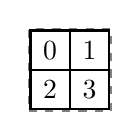
\begin{tikzpicture}
    \node[cell] at (0.5, 0.5) {};
    \foreach \x/\y [count=\i from 0] in {0/1,1/1,0/0,1/0} {
      \node[whitebox] at (\x,\y) {\i};
    }
  \end{tikzpicture}
  \caption{Cell pixels enumeration}
  \label{fig:pixelsEnumeration}
\end{figure}

We need also to define connectivity function for the condensed image.
We cannot actually just use 8-connectivity, as whether two cells are adjacent
cells of one CC depends not only on their coordinates, but also on their
configuration. See \autoref{fig:connectivity:examples} for examples.

\begin{figure}
  \centering
  \begin{subfigure}[t]{0.3\linewidth}
    \centering
    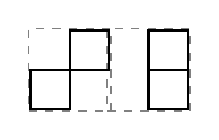
\begin{tikzpicture}
      \foreach \x in {0.5,2.5}
        \node[cell] at (\x,0.5){};
      \foreach \x/\y in {0/0, 1/1, 3/0, 3/1}
        \node[whitebox] at (\x, \y){};
    \end{tikzpicture}
    \caption{Nearby cells that are not directly connected.}
  \end{subfigure}
  \quad
  \begin{subfigure}[t]{0.3\linewidth}
    \centering
    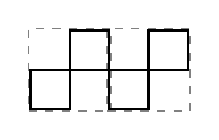
\begin{tikzpicture}
      \foreach \x in {0.5,2.5}
        \node[cell] at (\x,0.5){};
      \foreach \x/\y in {0/0, 1/1, 2/0, 3/1}
        \node[whitebox] at (\x, \y){};
    \end{tikzpicture}
    \caption{Directly connected cells.}
  \end{subfigure}
  \quad
  \begin{subfigure}[t]{0.3\linewidth}
    \centering
    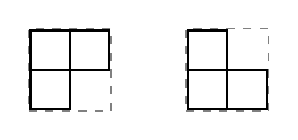
\begin{tikzpicture}
      \foreach \x in {0.5,4.5}
        \node[cell] at (\x,0.5){};
      \foreach \x/\y in {0/0, 0/1, 1/1, 4/0, 4/1, 5/0}
        \node[whitebox] at (\x, \y){};
    \end{tikzpicture}
    \caption{Cells that are not nearby in terms of 8-connectivity, cannot be
    directly connected.}
  \end{subfigure}
  \caption{Cells connectivity examples}
  \label{fig:connectivity:examples}.
\end{figure}

However, for every variant of relative placement of two nearby cells there is
a mask of pixels of each cells that are important for direct connectivity of
this pair of cells.
So two cells are considered directly connected, if they are nearby
in terms of 8-connectivity and each of them contains at least one object pixel
in the mask of important pixels corresponding to relative placement of the
cells. The masks are shown in \autoref{fig:connectivity:masks}.

\begin{figure}
  \centering
  \begin{subfigure}[t]{0.2\linewidth}
    \centering
    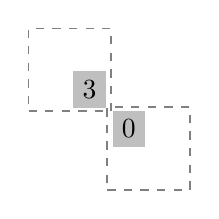
\begin{tikzpicture}
      \node[cell] at (0.5, 2.5) {};
      \node[cell] at (2.5, 0.5) {};
      \node[graybox] at (1, 2) {3};
      \node[graybox] at (2, 1) {0};
    \end{tikzpicture}
  \end{subfigure}
  \begin{subfigure}[t]{0.2\linewidth}
    \centering
    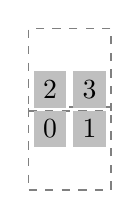
\begin{tikzpicture}
      \node[cell] at (0.5, 2.5) {};
      \node[cell] at (0.5, 0.5) {};
      \node[graybox] at (0, 2) {2};
      \node[graybox] at (1, 2) {3};
      \node[graybox] at (0, 1) {0};
      \node[graybox] at (1, 1) {1};
    \end{tikzpicture}
  \end{subfigure}
  \begin{subfigure}[t]{0.2\linewidth}
    \centering
    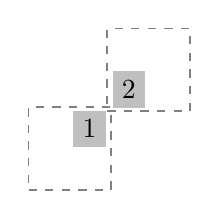
\begin{tikzpicture}
      \node[cell] at (0.5, 0.5) {};
      \node[cell] at (2.5, 2.5) {};
      \node[graybox] at (1, 1) {1};
      \node[graybox] at (2, 2) {2};
    \end{tikzpicture}
  \end{subfigure}
  \begin{subfigure}[t]{0.25\linewidth}
    \centering
    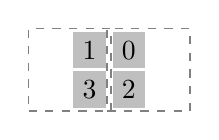
\begin{tikzpicture}
      \node[cell] at (0.5, 0.5) {};
      \node[cell] at (2.5, 0.5) {};
      \node[graybox] at (1, 0) {3};
      \node[graybox] at (1, 1) {1};
      \node[graybox] at (2, 0) {2};
      \node[graybox] at (2, 1) {0};
    \end{tikzpicture}
  \end{subfigure}
  \caption{Masks of important pixels for all four cases of relative placement
  of two nearby cells. Those pixels are filled in gray, with their numbers within
  cell specified.}
  \label{fig:connectivity:masks}
\end{figure}

The idea is that if we naturally encode mask pixels as 4-bit numbers in the
way similar to how we defined $c$, we can express the predicate denoting whether
two nearby cells
are directly connected efficiently with just two bitwise and one logical AND
operations.
As an example, \autoref{fig:connectivity:code} compares possible codes in \C
checking if the labels of the current pixel or cell and the one right on top of
it should be same for classic $8$-connectivity and for the new connectivity. Note
that as bitwise operations are usually relatively cheap, we added only a little
complication compared to decreasing the number of pixels to process by the
factor of $4$.

\begin{figure}
  \centering
  \begin{subfigure}[t]{0.475\linewidth}
    \centering
    \begin{lstlisting}
    if (b(x, y)) {
      if (b(x, y-1)) {
        // copy labels, or union label sets
      }
      // consider other directions
    }
    \end{lstlisting}
    \caption{Binary image with 8-connectivity.}
  \end{subfigure}
  \quad
  \begin{subfigure}[t]{0.475\linewidth}
    \centering
    \begin{lstlisting}
    if (c(x, y)) {
      if ((c(x, y-1) & ((1<<2) | (1<<3)))
       && (c(x, y)   & ((1<<0) | (1<<1)))) {
        // copy labels, or union label sets
      }
      // consider other directions
    }
    \end{lstlisting}
    \caption{Condensed image with new connectivity.}
  \end{subfigure}
  \caption{Checking the nearby top pixel/cell.}
  \label{fig:connectivity:code}
\end{figure}

\section{Benchmarks}

In this section we present performance benchmarks of some popular methods for
counting CC both with and without the $2 \times 2$ cells optimization.

\subsection{Algorithms overview}

As each of these methods, omitting DTSUF could be used with both condensed and
non-condensed images, for convenience we denote height and width of the image
on input of each algorithm as $H$ and $W$.

Also to avoid repeating ``pixel or cell'' we will just use the word ``pixel''
meaning the appropriate raster for non-condensed and condensed images.
When we mention neighbors of some pixel, we mean pixels that are directly
connected to it in terms of appropriate connectivity.

\subsubsection{DFS}

The first algorithm we chose for the benchmark is Depth First Search graph
traversal. Graph traversal algorithms are the general approach for CC labeling
in graphs, and DFS is arguably the most simple. Although not intended for image
labeling and suboptimal in most cases, it still has linear in the number of
pixels worst-case complexity in both time and memory.

Like most approaches, the algorithm has an outer loop over all pixels of the
image. Each time an object pixel (non-empty cell, in case it is actually a
cell) which is not labeled yet is encountered, DFS traversal is launched from
that pixel. The traversal labels all the object pixels of the same CC,
launching recursively from all unlabeled neighbors of current pixel.

\subsubsection{SUF}

Another general approach for graph CC labeling which is more popular in image
labeling is using some kind of a data structure to maintain disjoint sets of
pixels that are considered to be in the same CC.

The structure is commonly called Union-Find, as the two essential operations it
is supposed to support are Union, which is used to merge some two of the
disjoint sets in one, and Find, which is used to find the representative
element of the set some element belongs to, so that we can always tell if two
elements are in the same set. The structure can be implemented so that the
amortized time complexity for each operation is $O(\alpha(HW))$, where $\alpha$
is the inverse Ackermann function, and $\alpha(HW) < 5$ for all remotely
practical image sizes\cite{CLRS}. % TODO links

The approach that is named SUF (Scan plus Union-Find) in this paper follows.

Pixels are processed in the natural order: from top to bottom and from
left to right, so each row is fully processed before all rows after it.
So for each object pixel we encounter there are at most 4 nearby pixels
that were already processed, see \autoref{fig:suf:neighbors}.

At first each object pixel is considered to belong to its own CC, so right
before considering the neighbors we increment the CC counter. Moreover, it is
associated with its own disjoint set in the Union-Find structure. More
specifically, object pixel at position $x, y$ is associated with the set number
$xW + y$ to guarantee absence of collisions.

The possible neighbors are processed in the order shown on
\autoref{fig:suf:neighbors}, and for each neighbor that is object pixel, the
Union operation is performed on the two sets containing the current and the
neighbor pixel. In case the Union operation was successful, which means that
the pixels had belonged previously to different sets and we have just found a
way to merge two CC, the CC counter is decremented.

\begin{figure}
  \centering
  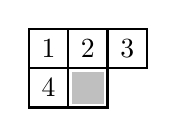
\begin{tikzpicture}
    \foreach \x/\y [count=\i from 1] in {0/1,1/1,2/1,0/0} {
      \node[whitebox] at (\x,\y) {\i};
    }
    \node[graybox] at (1, 0) {};
    \node[whitebox] at (1, 0) {};
  \end{tikzpicture}
  \caption{Neighbor mask for SUF algorithm family.}
  \label{fig:suf:neighbors}
\end{figure}

Note that this algorithm outputs not the matrix of final labels, but only the
number of CC. This is the place in which it differs from some common two-pass
approaches for CC % TODO references
labeling, as it is an algorithm not for labeling, but just for counting CC. The
latter is exactly what is needed for the aforementioned linear variation
problem.

Also we have to mention that for performance reasons the Union-Find internal
structures are allocated ahead to have the size of at least $HW$ to guarantee
that each object can be easily associated with unique starting set given only
its coordinates. So memory consumption of SUF is linear in the number of
pixels.

\subsubsection{SUF2}

This approach is a modification of SUF designed to reduce memory consumption
and potential number of cache-misses generated by Union-Find operations.

The idea is to run through each row twice: first time to establish label
equivalence classes within row, and the second time to set unique equal label
for all pixels of same CC. This gives us the opportunity to maintain just
$O(W)$ different labels at each moment, and so the Union-Find structure can be
allocated for only $O(W)$ elements, as opposed to $WH$ elements needed for SUF.

The exact maximum number of label equivalence classes between two adjacent rows
depends on whether the given image is condensed. For non-condensed images
$W=2M$, and maximum number of label equivalence classes in two adjacent rows is
$M=\frac{W}2$, as if two object pixels are both in adjacent rows and in
adjacent columns, then they are neighbors in terms of 8-connectivity.

On the other hand, for condensed images $W=M$, and maximum number of label
equivalence class in two adjacent rows of cells is $2W=2M$. See
\autoref{fig:suf2:extremal} for illustration on the extremal cases.

\begin{figure}
  \centering
  \begin{subfigure}{0.475\linewidth}
    \centering
    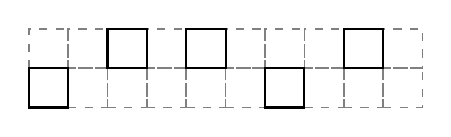
\begin{tikzpicture}
      \foreach \x in {0,1,...,9} \foreach \y in {0,1} {
        \node[whitebox,dashed,semithick,draw=gray] at (\x,\y) {};
      }
      \foreach \x/\y in {0/0,2/1,4/1,6/0,8/1} {
        \node[whitebox] at (\x,\y) {};
      }
    \end{tikzpicture}
    \caption{Non-condensed image, up to 5 different labels on 10 columns.}
  \end{subfigure}
  \quad
  \begin{subfigure}{0.475\linewidth}
    \centering
    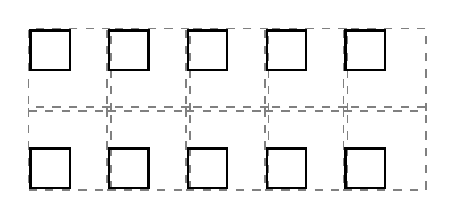
\begin{tikzpicture}
      \foreach \x in {0.5,2.5,...,8.5} \foreach \y in {0.5,2.5} {
        \node[cell] at (\x,\y) {};
      }
      \foreach \x in {0,2,...,8} \foreach \y in {0,3} {
        \node[whitebox] at (\x,\y) {};
      }
    \end{tikzpicture}
    \caption{Condensed image, up to 10 different labels on 5 columns.}
  \end{subfigure}
  \caption{Extremal cases for SUF2.}
  \label{fig:suf2:extremal}
\end{figure}

Our benchmarks show that, although SUF2 without condensation is generally more
efficient on noise images than SUF without condensation, the mentioned
consideration make the $2 \times 2$ optimization of SUF2 less dramatic in means
of performance increase factor. Optimized SUF2 significantly outperforms
optimized SUF only on huge noise images with less than $60\%$ density, while
falling behind on small and medium-sized noise images.

Note that, while SUF2 is intended for CC counting, its memory consumption is
only $O(W)$, which is significant for embedded systems and other resource-tight
applications.

\subsubsection{DTSUF}

This modification of SUF was implemented to compare the optimization we present
with another optimization suggested by Wu, Otoo and Suzuki\cite{wuotoo}, namely
decision tree. Unfortunately DTSUF (Decision Tree Scan plus Union-Find) is not
applicable for condensed image, as it exploits similar observations on
8-connectivity.

As before, the goal is to reduce the number of pixel lookup and label copy
operations. This is achieved with careful consideration of only the necessary
neighbors, stopping once the set of one or two label operations that are needed
is determined. The decision tree for processing an object pixel is shown on
\autoref{fig:dtsuf}.

\begin{figure}
  \centering
  \begin{subfigure}{0.3\linewidth}
    \centering
    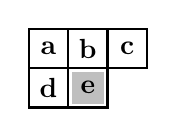
\begin{tikzpicture}
      \node[graybox] at (1,0) {};
      \foreach \x/\y/\a in {0/1/a,1/1/b,2/1/c,0/0/d,1/0/e} {
        \node[whitebox,font=\bf] at (\x,\y) {\a};
      }
    \end{tikzpicture}
    \caption{Neighbor enumeration.}
  \end{subfigure}
  \quad
  \begin{subfigure}{0.65\linewidth}
    \centering
    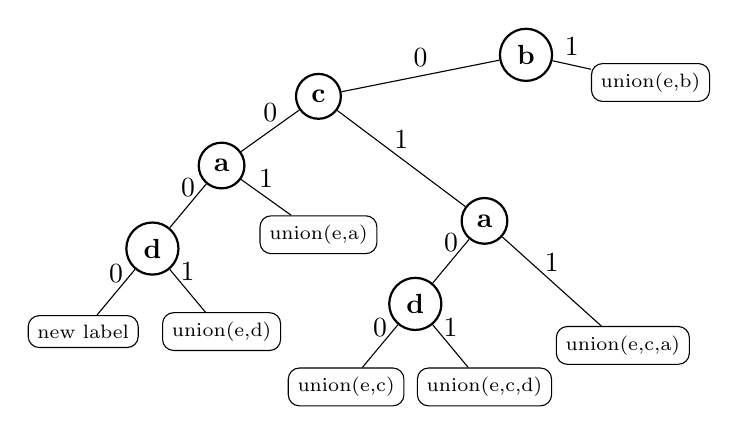
\begin{tikzpicture}[
      sibling distance=18em,
      lookup/.style = {shape=circle, draw, thick, align=center, font=\bf},
      action/.style = {shape=rectangle, rounded corners, draw, align=center, font=\scriptsize},
      result/.style = {font=\bf}
    ]
      \node[lookup] {b}
        child[level distance=3em,sibling distance=30em] {
          node[lookup] {c}
          child[level distance=5em, sibling distance=14em] {
            node[lookup] {a}
            child[level distance=6em, sibling distance=10em] {
              node[lookup] {d}
              child {
                node[action] {new label}
                edge from parent node[result,above] {$0$}
              }
              child {
                node[action] {union(e,d)}
                edge from parent node[result,above] {$1$}
              }
              edge from parent node[result,above] {$0$}
            }
            child {
              node[action] {union(e,a)}
              edge from parent node[result,above] {$1$}
            }
            edge from parent node[result,above] {$0$}
          }
          child[level distance=9em,sibling distance=24em] {
            node[lookup] {a}
            child[level distance= 6em, sibling distance=10em] {
              node[lookup] {d}
              child {
                node[action] {union(e,c)}
                edge from parent node[result,above] {$0$}
              }
              child {
                node[action] {union(e,c,d)}
                edge from parent node[result,above] {$1$}
              }
              edge from parent node[result,above] {$0$}
            }
            child[sibling distance=20em] {
              node[action] {union(e,c,a)}
              edge from parent node[result,above] {$1$}
            }
            edge from parent node[result,above] {$1$}
          }
          edge from parent node[result,above] {$0$}
        }
        child[level distance=2em] {
          node[action] {union(e,b)}
          edge from parent node[result,above] {$1$}
        };
    \end{tikzpicture}
    \caption{The decision tree.}
  \end{subfigure}
  \caption{DTSUF decision tree optimization.}
  \label{fig:dtsuf}
\end{figure}

\subsection{Condensation types}

\texten{
For memory-tight applications such as embedded systems it can be useful to
utilise the suggested condensation in a lazy way, so that without actually
constructing the condensed image we use a function (``view'') calculating color
of each cell with 4 lookups to the original binary image. This is probably most
interesting when combined with SUF2 algorithm, as it is a way to win some time
while avoiding memory footprint increase. However this lazy approach increases
the number of image lookups.
% So, according to our benchmark, this combination is efficient only for dense
% ($>30\%$) noise.
}\textru{
В некоторых случаях может быть более приемлемо использовать сжатие неявно, то
есть вместо построения 
}

So the benchmark charts show three levels of optimization applied to DFS, SUF
and SUF2: just method name in legend refers to method applied to non-condensed
image, ``+view'' means lazy memory-less condensation and ``+2x2'' means that a
temporary condensed image was constructed in memory. For the latter case, the
construction time was included into the overall measured time of run.

\subsection{Measurement}

For measurement purposes all algorithms and optimizations were implemented by us in \CXX.

The program was compiled using \texttt{g++ 5.3.0-3} compiler with \texttt{-O3}
optimization flag. All tests were run on same machine running under Arch Linux
with standard \texttt{linux 4.4.1-2} kernel, utilising non-overclocked
\texttt{Intel(R) Core(TM) i5-2430M CPU @ 2.40GHz} (L3 cache size 3072K)
processor and non-overclocked 1333MHz 8GiB Kingston RAM.

The test images were generated in the following manner. At first, for given
density $d$, the first $4dNM$ pixels of the $2N \times 2M$ image were filled
with object values, while rest filled with background values. Then all the
pixels were permuted using \texttt{std::shuffle} function from \CXX standard
library, which is an implementation of Fisher-Yates Shuffle
algorithm\cite{fisher:yates}.

All methods were run on same tests, which was achieved by supplying same seed
to the \texttt{std::mt19937} Mersenne Twister\cite{mt19937} random number
engine implementation from \CXX standard library before passing the engine to
\texttt{std::shuffle}.

\subsection{Results}

Line charts with benchmarks of mentioned algorithms on different noise images
are shown on
\Cref{fig:noise400x600,fig:noise800x1200,fig:noise1200x1800,fig:noise2000x3000,fig:noise4000x6000}.

The extremely bigger CPU time for SUF and DTSUF methods on huge images could be
explained by significant increase in the number of cache-misses produced by
Union-Find. The charts prove effectiveness of the $2 \times 2$ condensation
optimization.  

\newcommand{\inputtable}[2]{
  \begin{figure}
    \centering
    \includegraphics[height=0.45\textheight, keepaspectratio]{pics/#1x#2.eps}
    \caption{Average CPU time per run on noise images $#1 \times #2$ px.}
    \label{fig:noise#1x#2}
  \end{figure}
 % \begin{table}[p]
 %   \centering
 %   \input{tables/#1x#2}
 %   \caption{Average CPU time per run on noise images $#1 \times #2$ px}
 %   \label{tab:noise#1x#2}
 % \end{table}
}

% \inputtable{200}{300}
\inputtable{400}{600}
\inputtable{800}{1200}
\inputtable{1200}{1800}
\inputtable{2000}{3000}
\inputtable{4000}{6000}
% \inputtable{5000}{7500}

% \section{Summary and future work}


\begin{thebibliography}{5}

\bibitem {mak1}
Rudin, L., Osher, S., Fatemi, E.: Nonlinear total variation based noised removal algorithms. Phys. D. 60, 259-268 (1992)

\bibitem {mak2}
Kronrod, A.: On functions of two variables ," Uspehi Mat. Nauk 5, 1(35), 24-134(1950)

\bibitem {mak3}
Makovetskii, A., Kober, V.: Image restoration based on topological properties of functions of two variables.  Proc. SPIE Applications of Digital Image Processing XXXV, 8499, 84990A (2012)

\bibitem {mak4}
4.	Makovetskii, A., Kober, V.: Modified gradient descent method for image restoration. Proc. SPIE Applications of Digital Image Processing XXXVI, 8856, 885608-1 (2013)

\bibitem {mak5}
Chochia, P., Milukova, O.: Comparison of Two-Dimensional Variations in the Context of the Digital Image Complexity Assessment.  Journal of Communications Technology and Electronics, 2015, 60, no. 12,  pp. 1432-1440

\bibitem {hechao}
He, L., Chao, Y., Suzuki, K., Wu, K.:
Fast connected-component labeling. Pattern Recognition. v42, Pages 1977-1987. (2009)

%\bibitem {sterzh}
%Стержанов, М.:
%Методики выделения связных компонент в штриховых бинарных изображениях.
%Труды конференции ГрафиКон’2010. НИУ ИТМО. Санкт-Петербург. с. 169-174. (2010)

\bibitem {CLRS}
Cormen, H., Leiserson, E., Rivest, L., Stein, C.:
Introduction to Algorithms (Second ed.), MIT Press (2001)

\bibitem {wuotoo}
Wu, K, Otoo, E., Suzuki, K.:
Optimizing two-pass connected-component labeling algorithms.
Pattern Anal. Appl. (2008)

\bibitem {fisher:yates}
 Fisher, A., Yates, F.:
 Statistical tables for biological, agricultural and medical research (3rd ed.). 
 London: Oliver \& Boyd. pp. 26–27. OCLC 14222135 (1948)
 
\bibitem{mt19937}
Matsumoto, M., Nishimura, T.:
"Mersenne twister: a 623-dimensionally equidistributed uniform pseudo-random number generator".
ACM Transactions on Modeling and Computer Simulation 8 (1): 3–30. (1998)

\end{thebibliography}

\end{document}

